% begin module related-rates-ex1

\begin{frame} %[fragile]
\begin{example}
Air is being pumped into a spherical balloon such that \alertNoH{ 6}{its volume changes at a rate of 100 cm$^3$/s}.  \alertNoH{ 8}{How fast is the radius of the balloon increasing when the diameter is 50 cm?}
\begin{columns}[c]
\column{.6\textwidth}
\begin{itemize}
\item<2-> \textbf{Draw and introduce notation:}
\item<3->  At time $ t $ seconds, let\\
  $V=V(t) $ be the balloon's volume (cm$ ^3 $).
\item<4->  Let $r=r(t)$ denote its radius (cm).
\item<5->  \textbf{Identify given/req'd rates: }\\
Given: \alertNoH{ 6}{ $\uncover<6->{V'(t) = 100}$ \uncover<6->{cm$^3$/s.}}
\item<7->    Required:  \alertNoH{ 8}{\uncover<8->{$ r'(t)$ when $r = 25$ cm.}}
\end{itemize}
\column{.4\textwidth}
\abovedisplayskip=0pt
\belowdisplayskip=0pt
\abovedisplayshortskip=0pt
\belowdisplayshortskip=0pt
\uncover<2->{
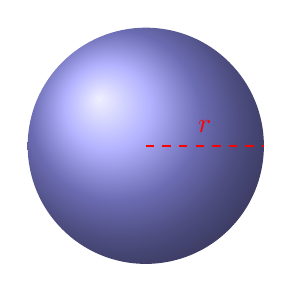
\begin{tikzpicture}
\shade [ball color=blue!40!white] (0,0) circle [radius=1.5cm];
\draw[color=red, dashed,  thick] (0,0) -- (1.5,0);
\node [below,color=red] at (.75,.45) {$r$};
\end{tikzpicture}
}
\end{columns}
\begin{itemize}
\item<9->  \textbf{Find an equation} relating the quantities with given/required rates.
\onslide<10->{
 \[ 
 V = \frac{4}{3}\pi r^3 \;\;\text{cm}^3
 \]
 }
\item<11->  Now: \textbf{Differentiate} (implicitly) this equation  with respect to time.
\end{itemize}
\end{example}
\end{frame}




\begin{frame} %[fragile]
\begin{example}
Air is being pumped into a spherical balloon such that \alertNoH{ 5}{its volume changes at a rate of 100 cm$^3$/s}.  \alertNoH{6}{How fast is the radius of the balloon increasing} when the \alertNoH{ 4}{diameter is 50 cm}?
\begin{align*}
V=\frac{4}{3}\pi r^3\;\;\;\;\longrightarrow\;\;\;\; 
V'(t)%
& =  \frac{\diff}{\diff t}\left( \frac{4}{3}\pi r^3\right)%
\\%
\uncover<2->{
&  { = } %
\frac{4}{3}\pi \cdot 3r^2\cdot \frac{\diff r}{\diff t}%
}\\%
\uncover<3->{
&  { = } %
4\pi r^2\cdot \frac{\diff r}{\diff t}%
}%
\end{align*}


\uncover<4->{
Now \textbf{evaluate} the above expression when  \alertNoH{ 4}{$ r=25 $}  and \alertNoH{ 5}{$ \diff V/\diff t = 100 $} in order to \alertNoH{ 6}{solve for $ \displaystyle \frac{\diff r}{\diff t} $}: \pause \pause 
\[
\frac{\diff r}{\diff t}=\frac{1}{4\pi r^2}\cdot\frac{\diff V}{\diff t} \uncover<7->{= \frac{1}{4\pi(25^2)}\cdot 100=\frac{1}{25\pi}\text{ cm/s}}
\]
}
\uncover<8->{%
Therefore the radius is increasing at a rate of $\frac{1}{ 25\pi}$ cm/s when $r = 25$ cm.
}%
\end{example}
\end{frame}

% end module related-rates-ex1
